\documentclass[journal,12pt,twocolumn]{IEEEtran}
\usepackage[utf8]{inputenc}
\usepackage{amssymb}
\usepackage{amsmath}
\usepackage{graphicx}

\newcommand{\myvec}[1]{\ensuremath{\begin{pmatrix}#1\end{pmatrix}}}
\title{AI1110 ASSIGNMENT-1}
\author{CS21BTECH11024 - Jonnala Varshini}

\begin{document}
\maketitle
\section*{ICSE 10 2018}
\section*{Question 7(c)}
\begin{center}
    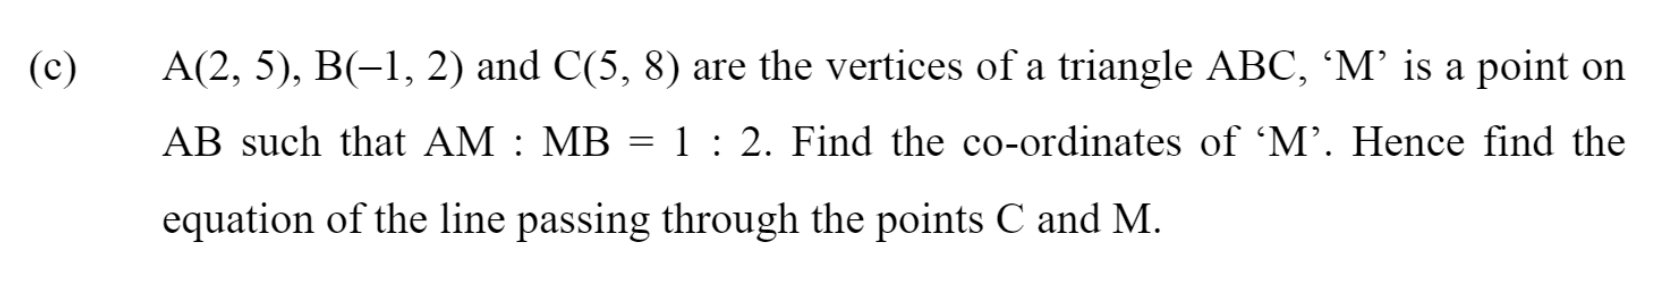
\includegraphics[scale=0.20]{prv1a.png}
\end{center}
\section*{Solution:}
According to the question, $M$ is a point on the side $AB$ such that $$AM : MB = 1 : 2$$
 When the line segment AB is divided internally by C in the ratio m:n, from Section formula,\\
 we get the Coordinates of point C as,\\
\begin{align*}
     [\myvec{\frac{mx2+nx1}{m+n}},\myvec{\frac{my2+ny1}{m+n}}], 
     where A\myvec{x1,y1}, B\myvec{x2,y2} \\
\end{align*}
From given data, using Section formula, we get
\begin{align*}
    M &= (\myvec{\frac{-1+4}{1+2}},\myvec{\frac{2+10}{1+2}})\\ 
    &= \myvec{1,4}
\end{align*}
The equation of the line joining two points (a,b),(c,d) is \\
\begin{align*}
    \myvec{y-b} = {\myvec{\frac{d-b}{c-a}}}\myvec{x-a}\\
\end{align*}
Here, the equation of the line joining $C(5,8)$ and $M(1,4)$ will be\\
\begin{align*}
    \myvec{y-4} = \myvec{\frac{8-4}{5-1}}\myvec{x-1} \\\\
\end{align*}
Simplified, we get the equation $$x-y+3=0$$

\subsection*{But, However,} On calculating, we get\\
The equation of the line joining A\myvec{2,5}, B\myvec{-1,2} as $x-y+3=0$ and \\
the equation of the line joining B\myvec{-1,2}, C\myvec{5,8} as $x-y+3=0$ too.\\

This implies that A,B,C are `collinear' and pass through $x-y+3=0$ and hence, given points $A,B,C$ don't form a triangle.\newline\\
Verified by plotting the graph of A,B,C and M points :
\begin{center}
  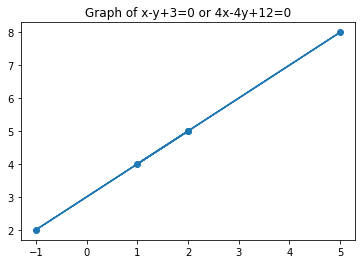
\includegraphics[scale=0.6]{prv1b.png}
\end{center}
    
\end{document}
